\documentclass[8pt]{beamer}
\usepackage{tikz}
\usepackage[utf8]{vietnam}
\usepackage{amsmath}
\usepackage{graphicx}
\usepackage{wrapfig}
\usepackage{hyperref}
\usepackage{mathrsfs}
\usepackage{verbatim}
\usetheme{Copenhagen}
\usecolortheme{dolphin}
\setbeamertemplate{navigation symbols}{}
\setbeamertemplate{headline}{}
\title[Chương 4: Thiết kế bộ lọc IIR] %optional
{Chương 4: Thiết kế bộ lọc IIR}
\subtitle{Xử lý tín hiệu số}
\author[Xử lý tín hiệu số] % (optional)
{Tín Vũ}
\date[VLC 2021] % (optional)
{tinvu1309@gmail.com}
\begin{document}
\frame{\titlepage}
\begin{frame}{Mục lục}
\tableofcontents
\end{frame}
\begin{frame}{Giới thiệu playlist}
\section{Giới thiệu playlist}
	\begin{itemize}
		\item Mình là Tín Vũ, hiện đang là sinh viên học tại Trường Đại học Công nghệ, Đại học Quốc gia Hà Nội. Mình tạo playlist video này để hỗ trợ các bạn học môn \textbf{Xử lý tín hiệu số}.
\item Khác với môn học tiên quyết \alert{Tín hiệu hệ thống} trước đó, bài giảng môn học này \textbf{hoàn toàn bám sát với đề cương và giáo trình nội bộ} của trường mình, nên các bạn trường khác cần phải lưu ý rất kĩ điều này.
\item Không chỉ dừng lại ở lý thuyết, playlist này \textbf{có bổ sung hướng dẫn lập trình cơ bản bằng GNU Octave/Matlab} để vẽ phổ tín hiệu, đáp ứng tần số và thiết kế bộ lọc.
\item Môn học này bao gồm \textbf{6 chương}, các chương đều liên quan rất chặt chẽ với nhau nên hãy học cẩn thận ngay từ \alert{Chương 0} để ôn thi cuối kì đỡ vất vả.
	\end{itemize}
\end{frame}
\begin{frame}{Tài liệu tham khảo}
\section{Tài liệu tham khảo}
\begin{itemize}
		\item Tài liệu tham khảo chính: Giáo trình Xử lý tín hiệu số (Nguyễn Linh Trung, Trần Đức Tân, Huỳnh Hữu Tuệ, ĐHCN, 2012).
		\item Tài liệu tham khảo phụ: Discrete-time Signal Processing (Alan V.Oppenheim, 2nd edition). 
	\end{itemize}
\end{frame}
\begin{frame}{Quy trình xử lý tín hiệu số}
\section{Quy trình xử lý tín hiệu số}
\begin{figure}[h]
			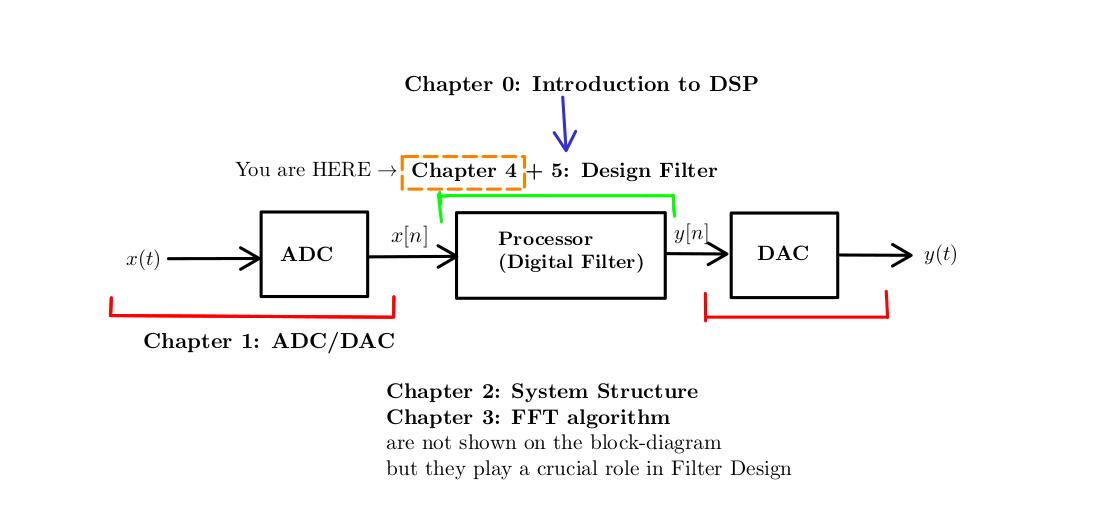
\includegraphics[width=1.1\textwidth]{1.jpg}
			\caption{DSP Learning Process}			\label{fig:re1}
		\end{figure}

\end{frame}
\begin{frame}{Thiết kế bộ lọc tương tự}
\section{Thiết kế bộ lọc tương tự}
\begin{itemize}
	\item Ý tưởng thiết kế bộ lọc tương tự 
\end{itemize}
\subsection{Ý tưởng thiết kế bộ lọc tương tự}
\subsubsection{Bộ lọc thông thấp (LP)}
\begin{itemize}
\item[-] Bộ lọc thông thấp (LP)
\end{itemize}
Ta bắt đầu khảo sát từ sơ đồ mạch của bộ lọc thông thấp (lowpass filter - LP) bậc 1 đơn giản nhất:
\begin{figure}[h]
			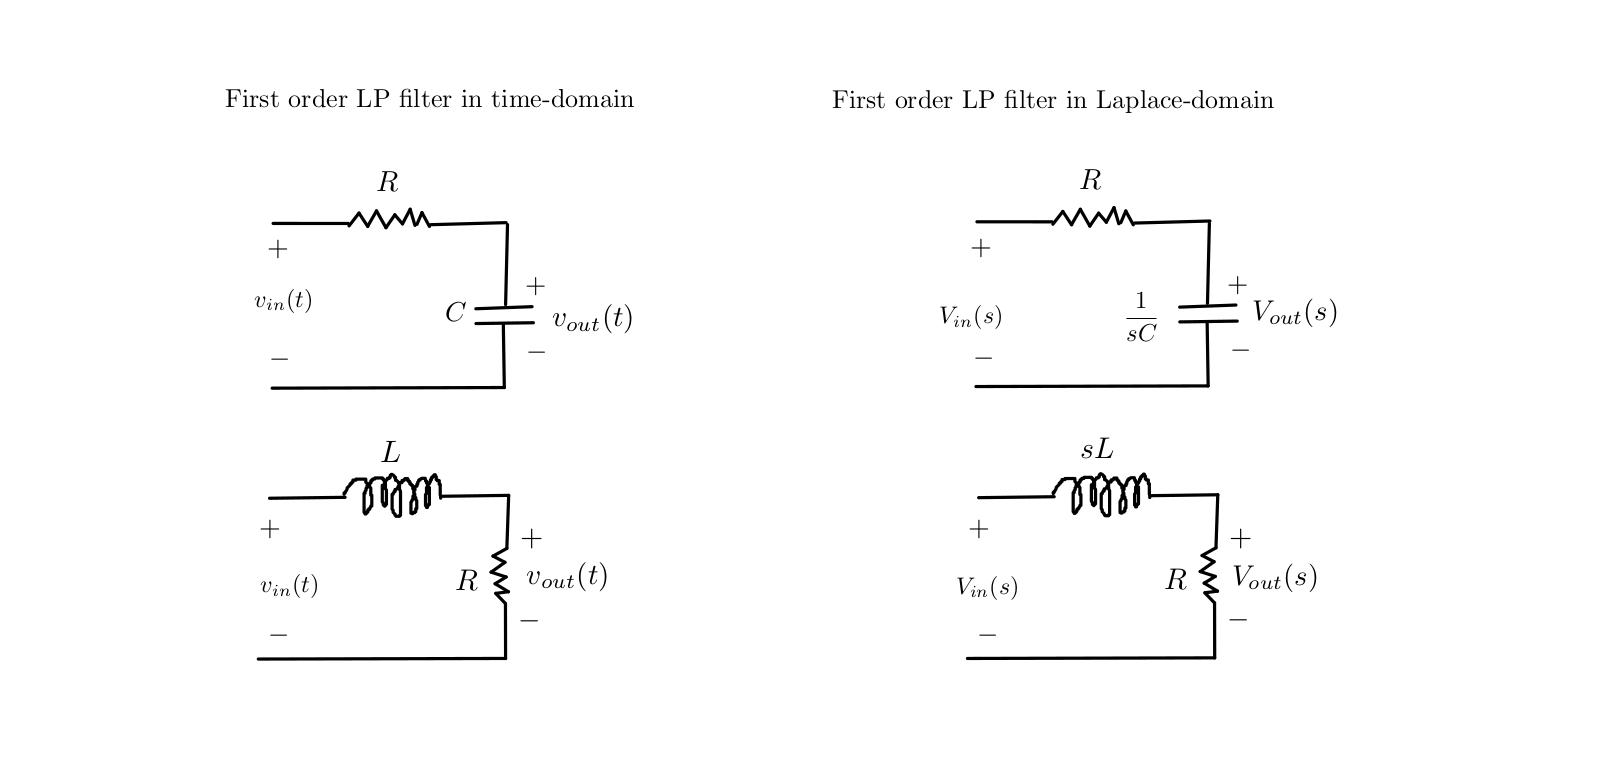
\includegraphics[width=1\textwidth]{2.jpg}
			\caption{First order LP filter in time and Laplace domain}			\label{fig:re2}
		\end{figure}

\end{frame}
\begin{frame}{Thiết kế bộ lọc tương tự}
Ta tìm hàm truyền của hai cấu trúc bộ lọc trên:
$$H(s)=\frac{\frac{1}{sC}}{R+\frac{1}{sC}}=\frac{1}{sRC+1}$$
$$H(s)=\frac{R}{R+sL}=\frac{1}{s\frac{L}{R}+1}$$
Ta đặt $\tau=RC$ hoặc $\tau=\frac{L}{R}$ là hằng số thời gian (time constant), ta thấy cả hai hàm truyền đều có chung dạng công thức: $$H(s)=\frac{1}{s\tau+1}$$
Ta muốn tìm đáp ứng tần số của hệ thống (bộ lọc là hệ thống nhân quả ổn định), thay $s=j\Omega$, ta có:
$$H(j\Omega)=\frac{1}{j\Omega\tau+1}\Rightarrow |H(j\Omega)|=\frac{1}{\sqrt{1+(\Omega\tau)^2}}$$
Hiển nhiên: $$H(j\Omega)=\frac{1}{j\Omega\tau+1}=\frac{1-j\Omega\tau}{1+(\Omega\tau)^2}\Rightarrow \angle H(j\Omega)=-\arctan{(\Omega\tau)}$$
Ta muốn biểu diễn đáp ứng tần số và đáp ứng pha của bộ lọc bằng \textbf{thang tuyến tính} và \textbf{thang dB}.
\end{frame}
\begin{frame}{Thiết kế bộ lọc tương tự}
\begin{figure}[h]
			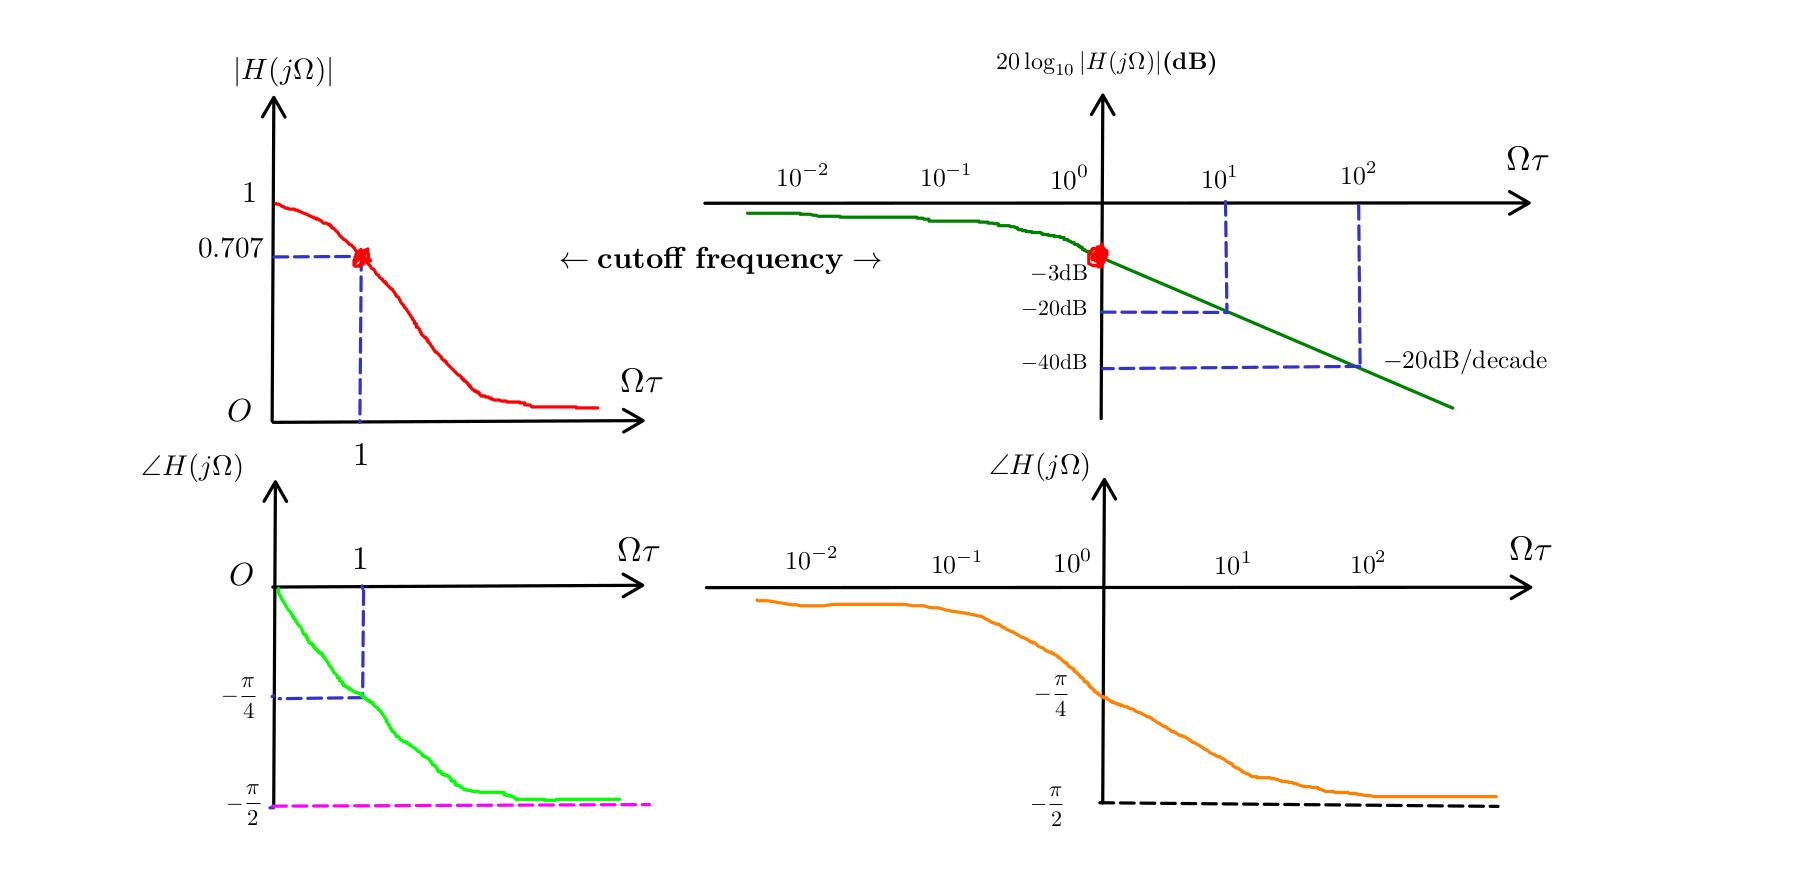
\includegraphics[width=1.1\textwidth]{3.jpg}
			\caption{First order LP filter in linear and dB scale}			\label{fig:re2}
		\end{figure}

\end{frame}
\begin{frame}{Thiết kế bộ lọc tương tự}
	Ta thấy rằng bộ lọc thông thấp (từ giờ ta sẽ gọi tắt các bộ lọc theo thuật ngữ tiếng Anh) LP có độ lợi $G=-20$dB/decade (gain), và tín hiệu sau khi đi qua bộ lọc có hiện tượng \textbf{méo pha} được thể hiện rất rõ trên phổ. Đối với bộ lọc tương tự đơn giản, ta \alert{không thể khắc phục được hiện tượng méo pha}, ta chỉ có thể cải thiện giá trị \textbf{độ lợi G} mà thôi.

	\\Đối với bộ lọc tương tự đơn giản, ta định nghĩa khái niệm hằng số \textbf{tần số cắt} (cutoff frequency) chính là \alert{tần số biên}, tại giá trị này \textbf{năng lượng} của tín hiệu gốc bị \textbf{suy hao một nửa}. 
	\\ Nếu ta quy đổi theo thang dB, độ lợi $G_{c}$ tại tần số cắt là:
	$$G_{c}=20\log_{10}\left(\frac{1}{\sqrt{1+1}}\right)=-3\text{dB}$$
	Từ đáp ứng biên độ của bộ lọc LP bậc 1: $$|H(j\Omega)|=\frac{1}{\sqrt{1+(\Omega\tau)^2}}$$
	 Để giảm độ lợi $G$ xuống càng thấp càng tốt, ta thiết kế bộ lọc LP có bậc $n$ tổng quát có phương trình đáp ứng biên độ như sau:
	 $$|H(j\Omega)|=\frac{1}{\sqrt{1+(\Omega\tau)^{\alert{2n}}}}$$
	 Ta giới thiệu một vài sơ đồ mạch bộ lọc tương tự LP có bậc $n=2$ và dạng tổng quát (Cauer form). \textbf{Lưu ý: bậc bộ lọc bằng số phần tử dự trữ năng lượng trong mạch}.
\end{frame}
\begin{frame}{Thiết kế bộ lọc tương tự}
\begin{figure}[h]
			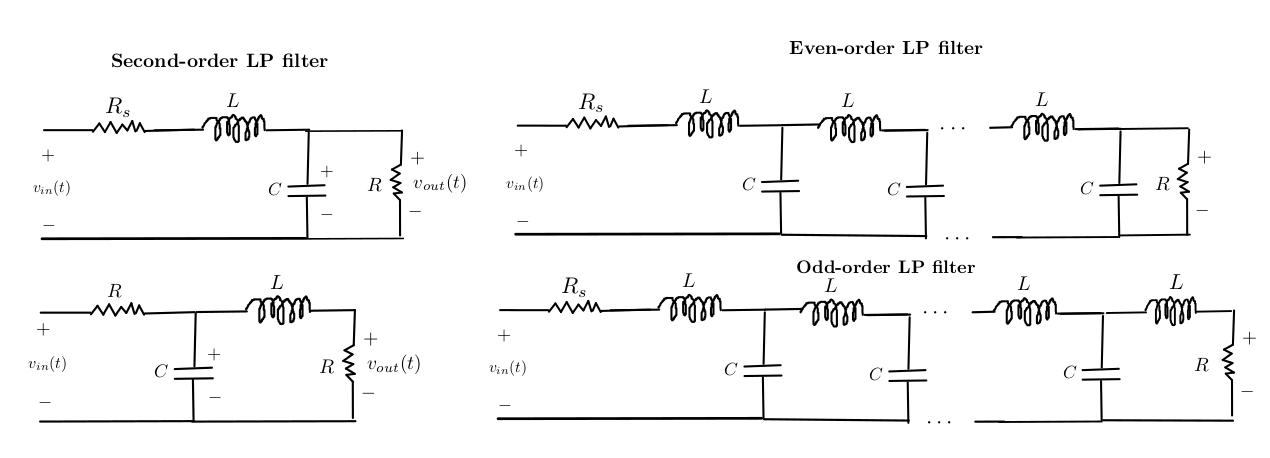
\includegraphics[width=1.1\textwidth]{4.jpg}
			\caption{Second order LP filter and higher order in Cauer form}			\label{fig:re2}
		\end{figure}

\end{frame}
\begin{frame}{Thiết kế bộ lọc tương tự}
\begin{figure}[h]
			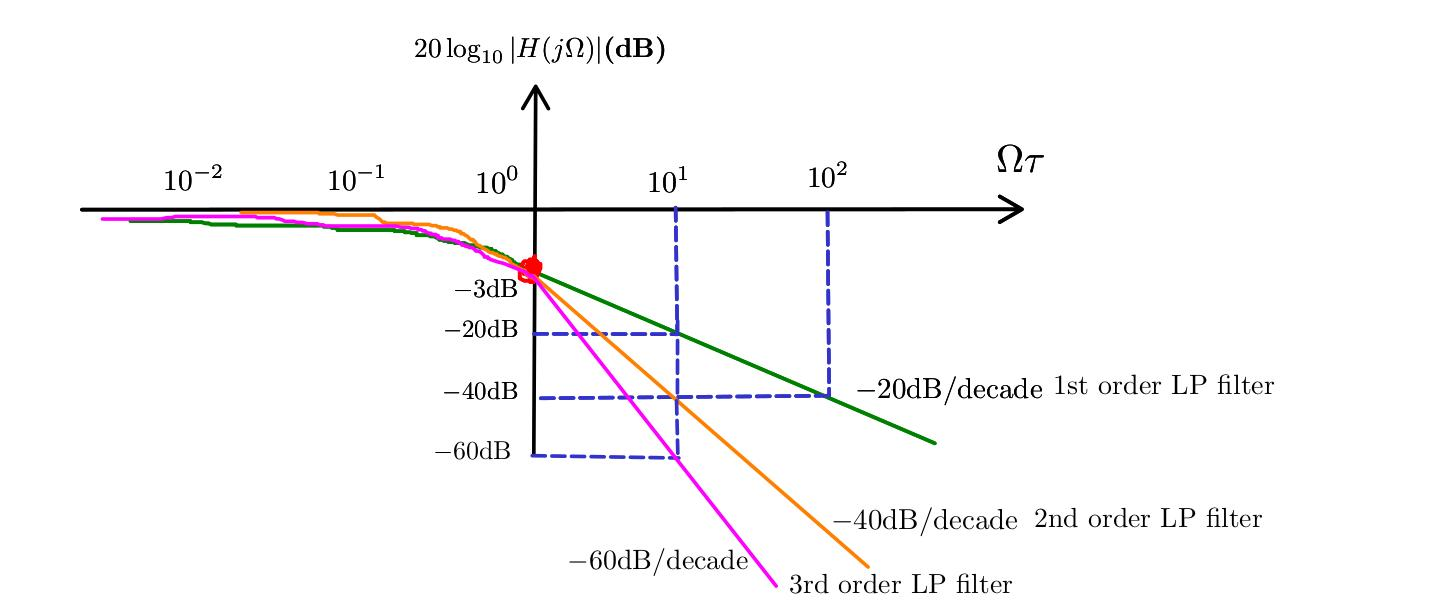
\includegraphics[width=1.1\textwidth]{5.jpg}
			\caption{Frequency response in dB scale of high order LP filter}			\label{fig:re2}
		\end{figure}

\end{frame}
\begin{frame}{Thiết kế bộ lọc tương tự}
\begin{itemize}
	\item[-] Bộ lọc thông cao (HP)
\end{itemize}
\subsubsection{Bộ lọc thông cao (HP)}
Cũng tương tự như bộ lọc LP, ta bắt đầu từ việc khảo sát bộ lọc HP bậc 1 đơn giản nhất có sơ đồ mạch như sau:
\begin{figure}[h]
			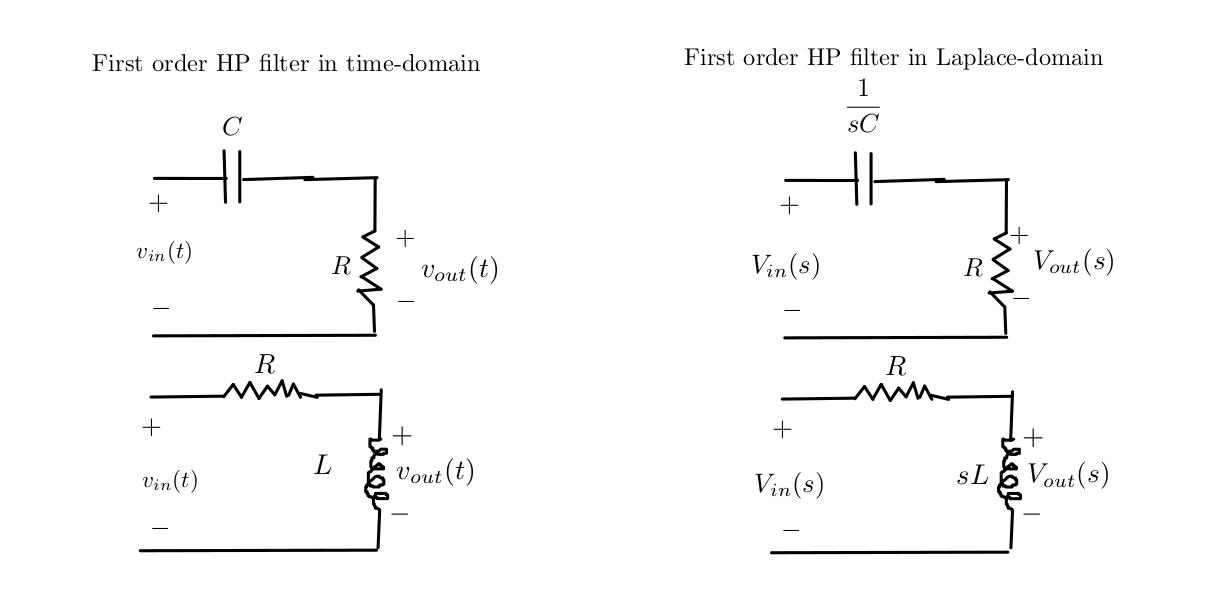
\includegraphics[width=1.1\textwidth]{6.jpg}
			\caption{First order HP filter in time and Laplace domain}			\label{fig:re2}
		\end{figure}

\end{frame}
\begin{frame}{Thiết kế bộ lọc tương tự}
Ta cũng xây dựng được biểu thức hàm truyền của hai bộ lọc HP trên như sau:
$$H(s)=\frac{R}{R+\frac{1}{sC}}=\frac{sRC}{sRC+1}$$
$$H(s)=\frac{sL}{sL+R}=\frac{s\frac{L}{R}}{s\frac{L}{R}+1}$$
Đặt $\tau=RC$ hay $\tau=\frac{L}{R}$ là hằng số thời gian (time constant), ta thu được dạng hàm truyền của bộ lọc HP: $$H(s)=\frac{s\tau}{s\tau+1}$$
Hiển nhiên đây là hệ thống nhân quả ổn định, ta thay $s=j\Omega$ để tìm đáp ứng tần số của bộ lọc HP: $$H(j\Omega)=\frac{j\Omega\tau}{j\Omega\tau+1}\Rightarrow |H(j\Omega)|=\frac{\Omega\tau}{\sqrt{(\Omega\tau)^2+1}}=\frac{1}{\sqrt{1+\left(\frac{1}{\Omega\tau}\right)^2}}$$
Dễ thấy: $$H(j\Omega)=\frac{j\Omega\tau(1-j\Omega\tau)}{1+(\Omega\tau)^2}=\frac{(\Omega\tau)^2+j\Omega\tau}{1+(\Omega\tau)^2}\Rightarrow\angel \angle H(j\Omega)=\arctan{\frac{1}{\Omega\tau}}$$
Tương tự, ta cũng vẽ đồ thị đáp ứng biên độ và pha của bộ lọc HP bằng thang tuyến tính và thang dB.
\end{frame}
\begin{frame}{Thiết kế bộ lọc tương tự}
\begin{figure}[h]
			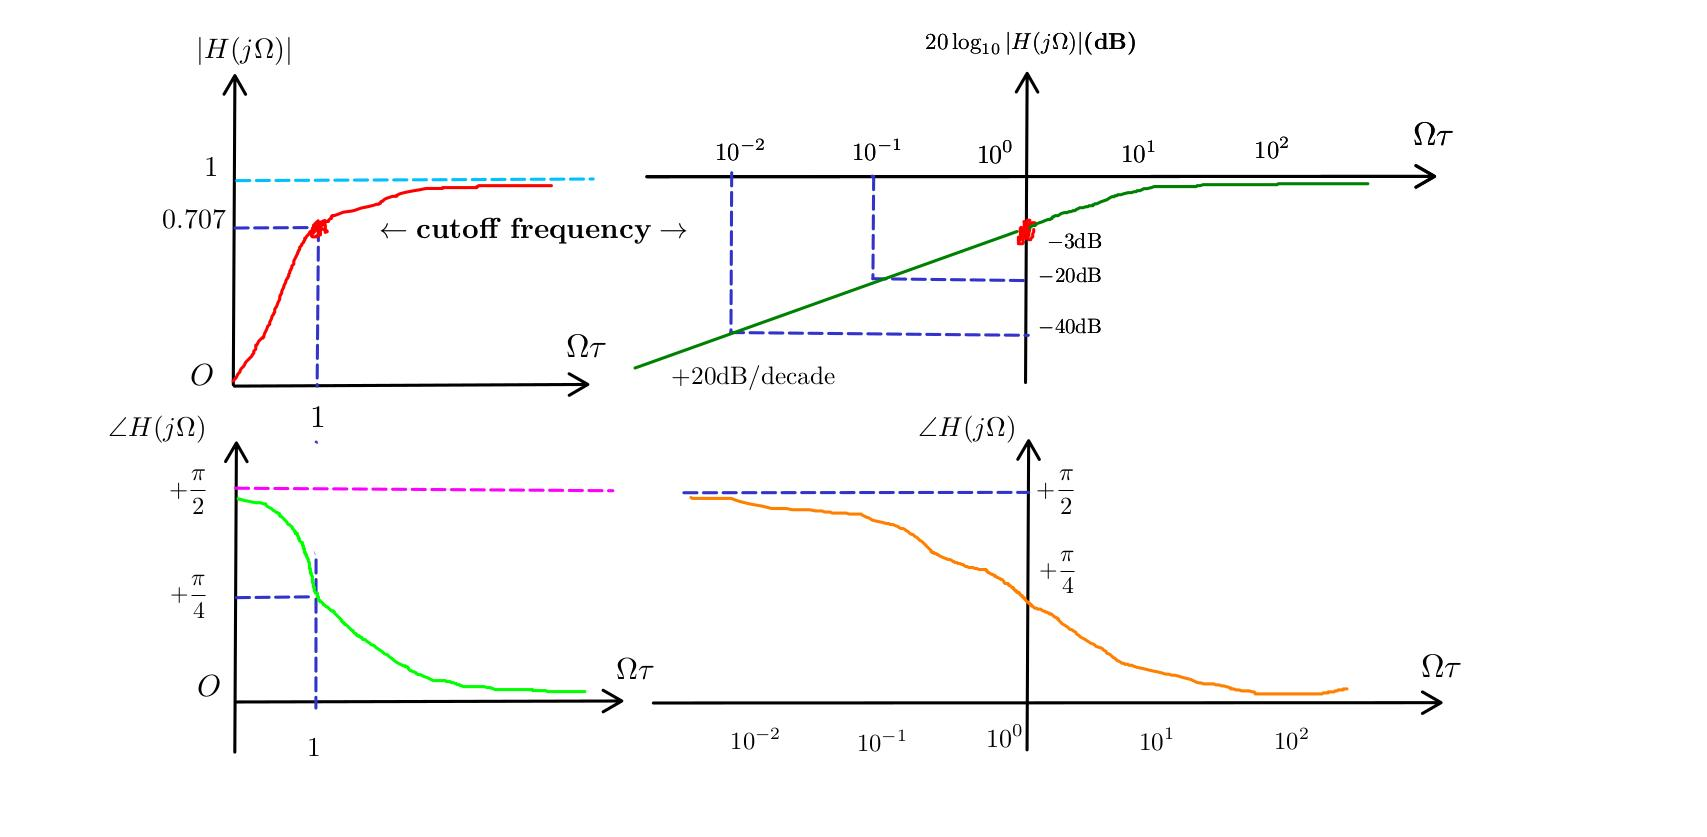
\includegraphics[width=1.1\textwidth]{7.jpg}
			\caption{First order HP filter in linear and dB scale}			\label{fig:re2}
		\end{figure}

\end{frame}
\begin{frame}{Thiết kế bộ lọc tương tự}
Tương tự với bộ lọc LP, tần số cắt cũng nằm tại vị trí $-3$dB. Từ phương trình đáp ứng biên độ của bộ lọc HP bậc 1:  $$|H(j\Omega)|=\frac{1}{\sqrt{1+\left(\frac{1}{\Omega\tau}\right)^{2}}}$$
Ta cũng có phương trình đáp ứng biên độ của bộ lọc HP bậc $n$ tổng quát:
$$|H(j\Omega)|=\frac{1}{\sqrt{1+\left(\frac{1}{\Omega\tau}\right)^{2n}}}$$
Dễ thấy bộ lọc HP \alert{chính là phiên bản "đảo ngược"} của bộ lọc LP. Đây là nhận định cực kì quan trọng đóng vai trò cơ sở cho thuật toán thiết kế bộ lọc HP được nghiên cứu sau này.
\\ Ta giới thiệu một vài sơ đồ mạch tương tự cấu trúc bộ lọc HP bậc 2 và cao hơn như dưới đây. \textbf{Lưu ý: cũng giống như bộ lọc LP, bậc bộ lọc bằng số phần tử dự trữ năng lượng trong mạch.}
\end{frame}
\begin{frame}{Thiết kế bộ lọc tương tự}
\begin{figure}[h]
			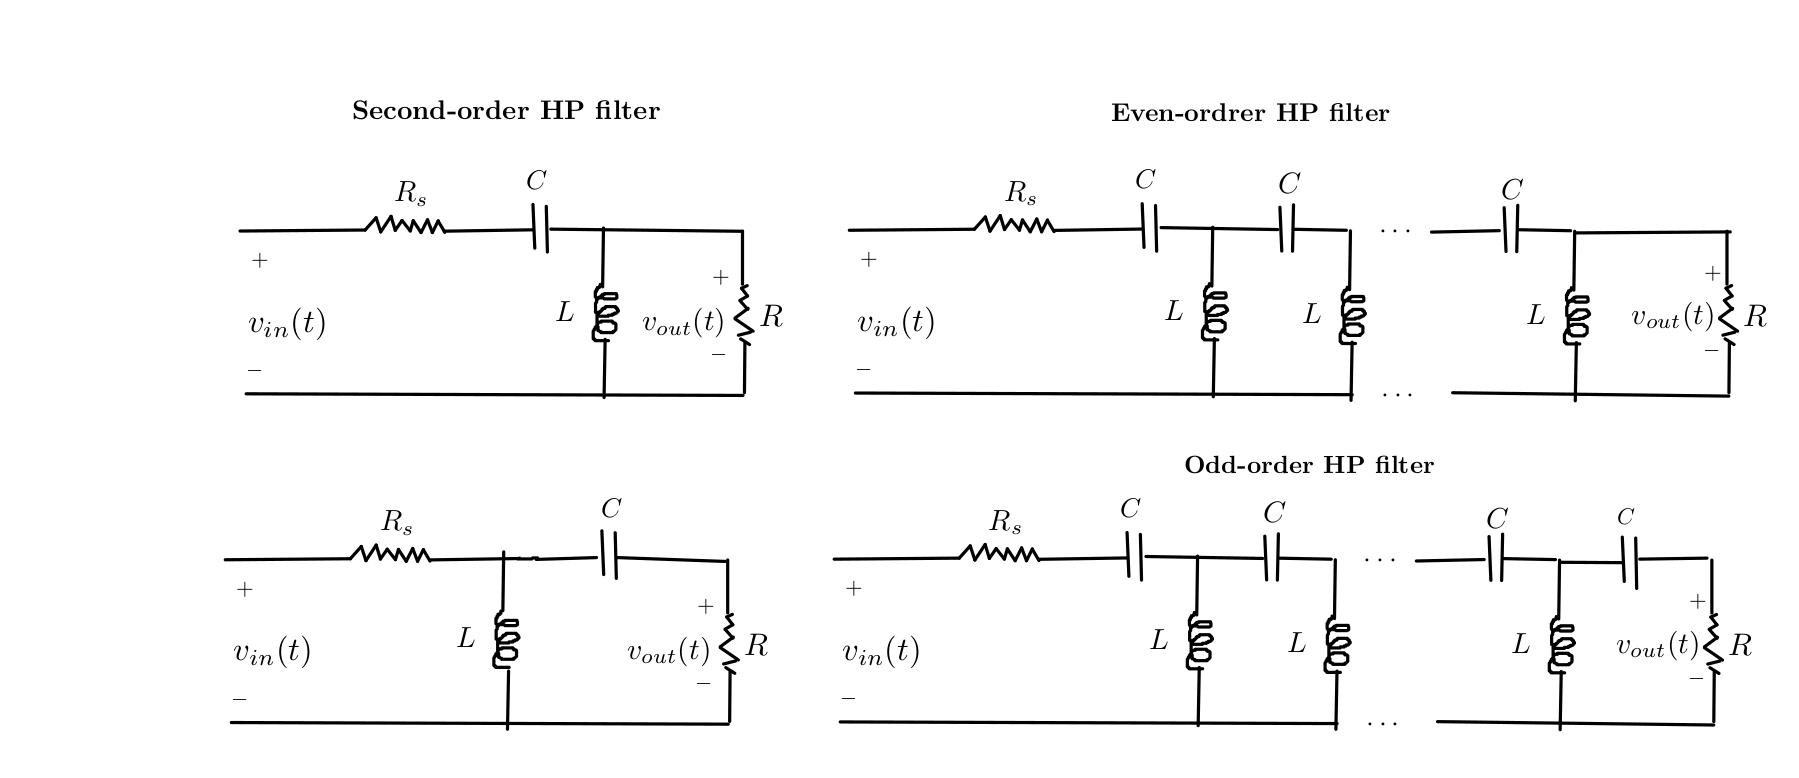
\includegraphics[width=1.1\textwidth]{8.jpg}
			\caption{Second order HP filter and higher in Cauer form}			\label{fig:re2}
		\end{figure}


\end{frame}
\begin{frame}{Thiết kế bộ lọc tương tự}
\begin{figure}[h]
			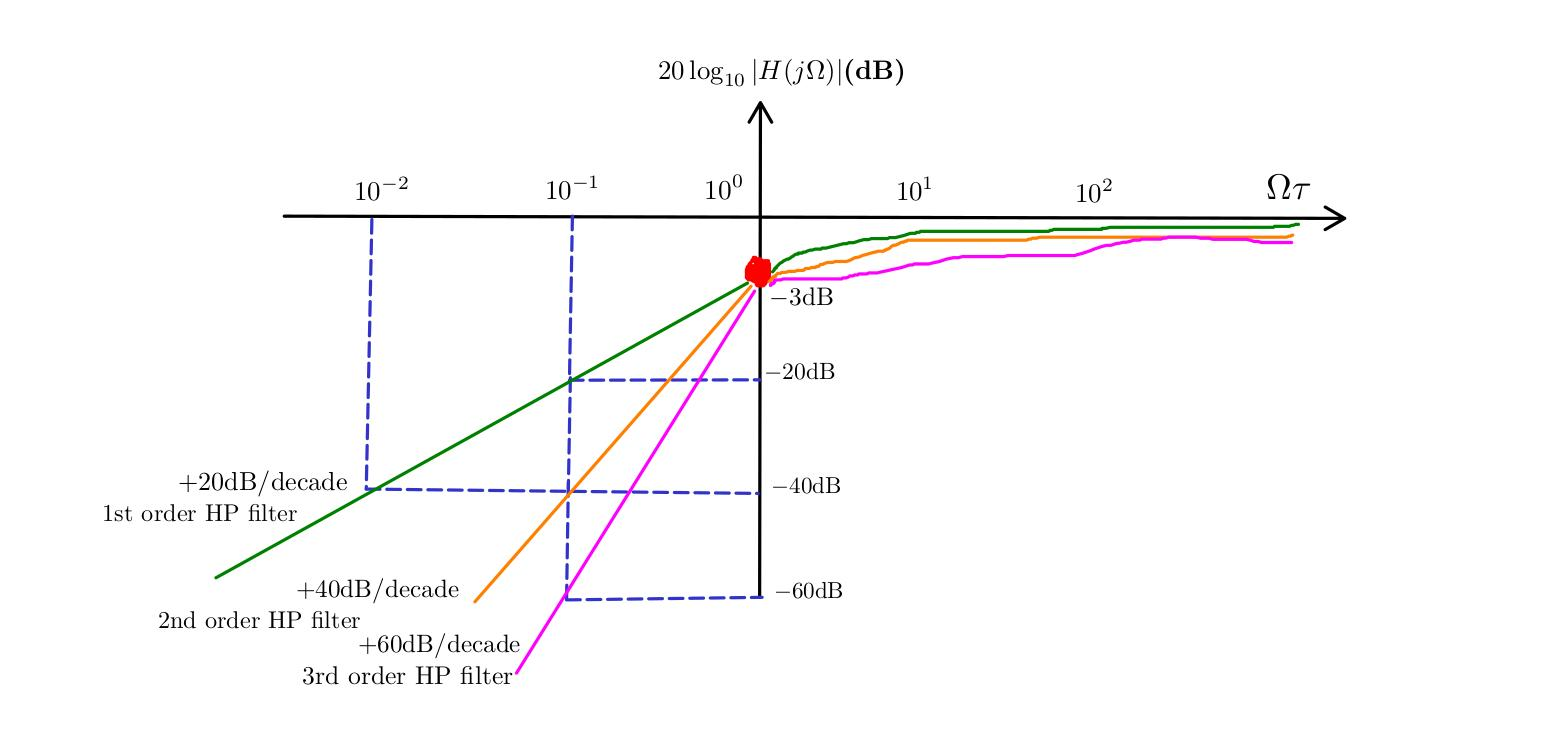
\includegraphics[width=1.1\textwidth]{9.jpg}
		\caption{Frequency response in dB scale of high order HP filter}			\label{fig:re2}
		\end{figure}

\end{frame}
\begin{frame}{Thiết kế bộ lọc tương tự}
\subsubsection{Bộ lọc thông dải (BP)}
\begin{itemize}
	\item[-] Bộ lọc thông dải (BP)
\end{itemize}

\begin{figure}[h]
			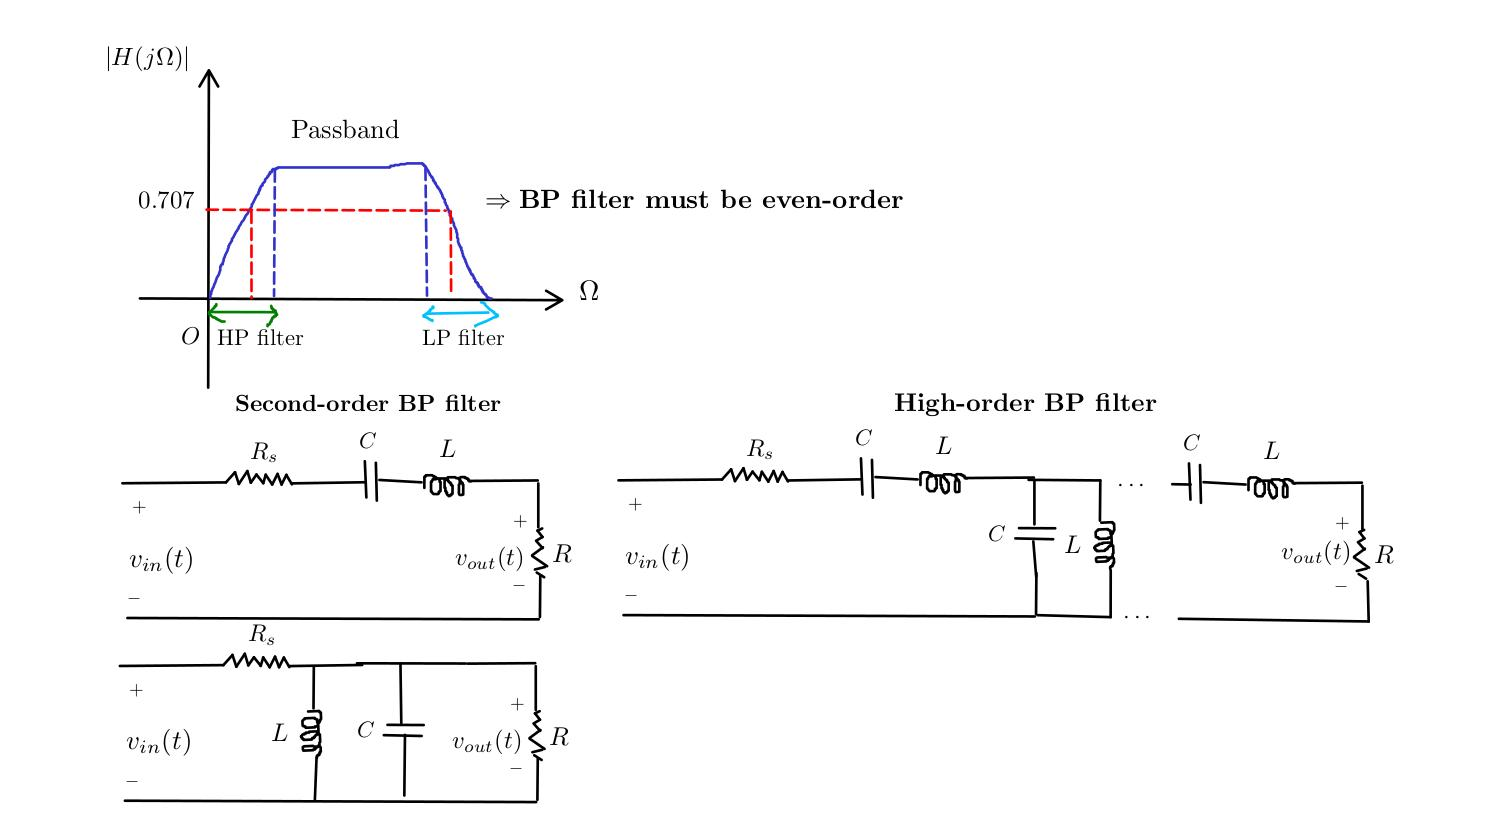
\includegraphics[width=1.1\textwidth]{10.jpg}
		\caption{Bandpass filter}			\label{fig:re2}
		\end{figure}
\end{frame}
\begin{frame}{Thiểt kế bộ lọc tương tự}
\begin{itemize}
	\item[-] Bộ lọc chặn dải (BS)
\end{itemize}
\subsubsection{Bộ lọc chặn dải (BS)}
\begin{figure}[h]
			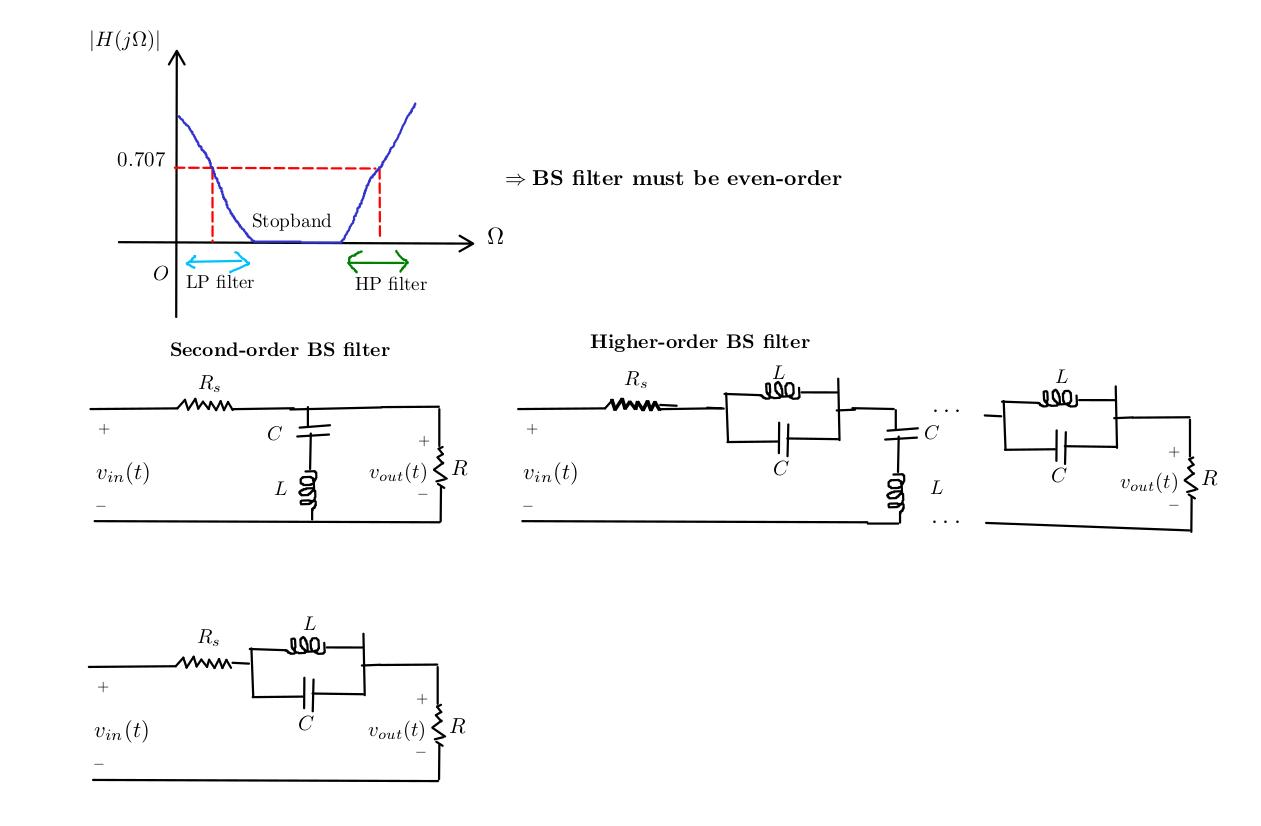
\includegraphics[width=1\textwidth]{11.jpg}
		\caption{Bandstop filter}			\label{fig:re2}
		\end{figure}

\end{frame}
\begin{frame}{Thiết kế bộ lọc tương tự}
\subsection{Thiết kế bộ lọc LP}
\subsubsection{Bộ lọc Butterworth}
\begin{itemize}
	\item Thiết kế bộ lọc LP
\end{itemize}

Bộ lọc LP là loại bộ lọc \textbf{dễ thiết kế nhất} và là \alert{bộ lọc cơ sở để thiết kế các loại bộ lọc khác}. Ta giới thiệu 2 họ bộ lọc tương tự LP cơ bản nhất trong giới hạn chương trình học phần, đó là \textbf{bộ lọc Butterworth} và \textbf{bộ lọc Chebyshev}.
\begin{itemize}
	\item[-] Bộ lọc Butterworth
\end{itemize}
Bộ lọc LP Butterworth là loại bộ lọc đơn giản nhất có đáp ứng biên độ tổng quát:
$$|H(j\Omega)|=\frac{1}{\sqrt{1+\left(\frac{\Omega}{\Omega_{c}}\right)^{2n}}}\Rightarrow |H^{2}(j\Omega)|=\frac{1}{1+\left(\frac{\Omega}{\Omega_{c}}\right)^{2n}}$$
với $\Omega_{c}$ là \alert{tần số cắt của bộ lọc} tại độ lợi \alert{$G_{c}=-3$dB}, và $n$ là \textbf{bậc của bộ lọc}.
\\ Ta rất dễ nhận ra rằng, phương trình đáp ứng biên độ của họ bộ lọc LP Butterworth \textbf{giống} với dạng đáp ứng biên độ bộ lọc LP được thiết kế bằng các linh kiện điện tử thụ động đơn giản $R,L,C$ đã phân tích ở trên.
\\ Hay nói cách khác, phương trình đáp ứng biên độ của bộ lọc LP Butterworth \textbf{lấy ý tưởng từ phương pháp thiết kế bộ lọc LP thụ động đơn giản}.
\\ Ta biểu diễn đáp ứng biên độ của bộ lọc LP như sau:
\end{frame}
\begin{frame}{Thiết kế bộ lọc tương tự}
\begin{figure}[h]
			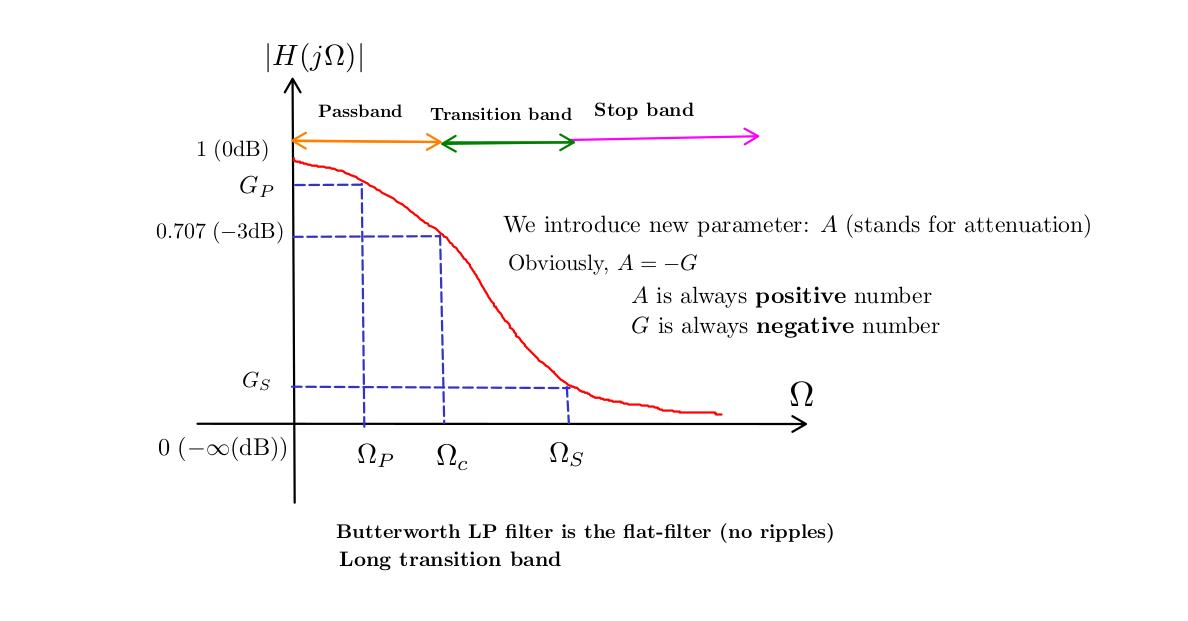
\includegraphics[width=1\textwidth]{12.jpg}
		\caption{Frequency response of Butterworth LP filter}			\label{fig:re2}
		\end{figure}

\end{frame}
\begin{frame}{Thiết kế bộ lọc tương tự}
	Bản chất của bài toán thiết kế bộ lọc là tìm \alert{hàm truyền $H(s)$} của hệ thống từ công thức đáp ứng tần số $|H(j\Omega)|$. Sau đó từ hàm truyền tìm được, người ta sẽ sử dụng các linh kiện điện tử phù hợp như $R,L,C$ hay Op-Amp để lắp ráp bộ lọc tương ứng.
\\ Để dễ dàng hình dung hơn về quy trình thiết kế bộ lọc, ta sẽ xét 3 ví dụ cơ bản sau:
\begin{enumerate}
	\item[1] Thiết kế bộ lọc Butterworth LP bậc 1 có tần số cắt $\alert{\Omega_{C}=1\;\text{(rad/s)}}$.
Từ phương trình đáp ứng tần số (thực ra đáp ứng biên độ là tên gọi chính xác hơn về thuật ngữ), ta có:
$$|H(j\Omega)|=\frac{1}{\sqrt{1+\Omega^2}}\Rightarrow |H^2(j\Omega)|=\frac{1}{1+\Omega^2}$$
Do bộ lọc là hệ thống ổn định, nên ta luôn có $\alert{s=j\Omega}$. Từ công thức tích liên hợp phức cơ bản, ta có kết quả rất quan trọng: $$\alert{|H^2(j\Omega)|=H(j\Omega)H(j\Omega)^*=H(j\Omega)H(-j\Omega)=H(s)H(-s)}$$
Thay toàn bộ $s$ vào phương trình đáp ứng tần số, ta thu được:
$$|H^2(j\Omega)|=\frac{1}{1+\Omega^2}\Rightarrow H(s)H(-s)=\frac{1}{1+\left(\frac{s}{j}\right)^2}=\frac{1}{-s^2+1}$$
Giải phương trình điểm cực của $H(s)H(-s)$, ta thu được $2$ điểm cực $s=\pm 1$, thế nhưng ta muốn tìm \alert{hàm truyền $H(s)$} có nghiệm cực sao cho đảm bảo \textbf{hệ thống ổn định}, tương đương với $\Re{(s)}<0$. Vậy ta chọn nghiệm cực $s=1$ và thu được hàm truyền: $$H(s)=\frac{1}{s+1}$$
	\end{enumerate}

\end{frame}
\begin{frame}{Thiết kế bộ lọc tương tự}
	\begin{enumerate}
		\item[2] Thiết kế bộ lọc Butterworth LP bậc 2 có tần số cắt $\alert{\Omega_{C}=1\;\text{(rad/s)}}$.  Thực hiện với quy trình tương tự, ta cũng có:

$$|H(j\Omega)|=\frac{1}{\sqrt{1+\Omega^4}}\Rightarrow |H^2(j\Omega)|=\frac{1}{1+\Omega^4}$$
Thay $s=j\Omega$, ta cũng có:

$$|H^2(j\Omega)|=\frac{1}{1+\Omega^4}\Rightarrow H(s)H(-s)=\frac{1}{1+\left(\frac{s}{j}\right)^4}=\frac{1}{s^4+1}$$
	\end{enumerate}
\end{frame}
\end{document}
